\section{Storage Management}

\subsection{Introduction}

A big part of the performance of databases arises from proper storage management (movement through hierarchy), adequate data representations and suitable optimizations on organizing the data in memory and disk.

Databases provide the illusion of large memory capacity and try to hide the performance problems created by implementing desirable properties (high bandwidth for sequential and concurrent access, low latencies for random accesses, persistent, etc.) through complex architectures and optimizations. Two key guarantees we want to have provided by a DB storage system are: persistent and recoverable data (even in the event of a failure). We would also like physical data independence.



\subsection{Memory Hierarchy}

Databases go through the entire memory hierarchy frequently. Enhance locality (data organization, query scheduling), make sure data is available at layer where it is needed (pre-fetching), be clever about what to keep at each layer (caching, replacement) and keep track of modifications and write back to the lower layers (to persistent storage) when needed.

\begin{figure}[h]
	\centering
	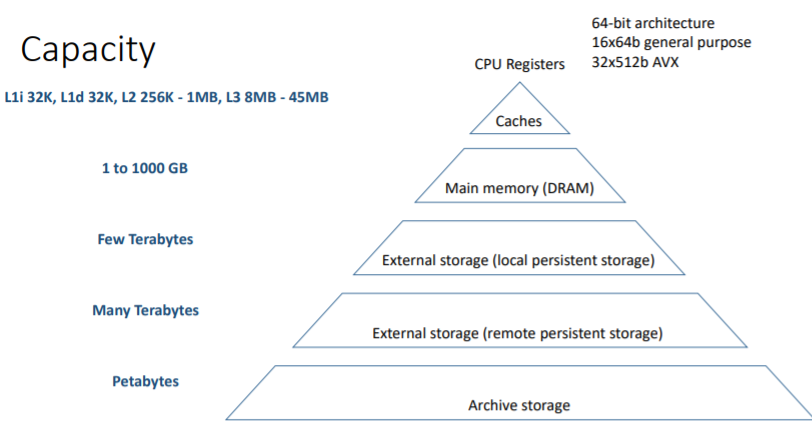
\includegraphics[scale=0.5]{images/1-cap.PNG}
	\caption{Memory hierarchy capacities.}
	\label{fig:cap}
\end{figure}

\begin{figure}[h]
	\centering
	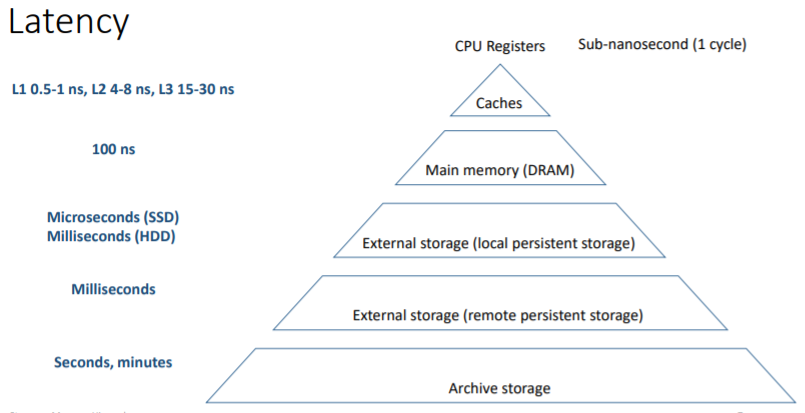
\includegraphics[scale=0.5]{images/1-lat.PNG}
	\caption{Memory hierarchy latencies.}
	\label{fig:lat}
\end{figure}

\begin{figure}[h]
	\centering
	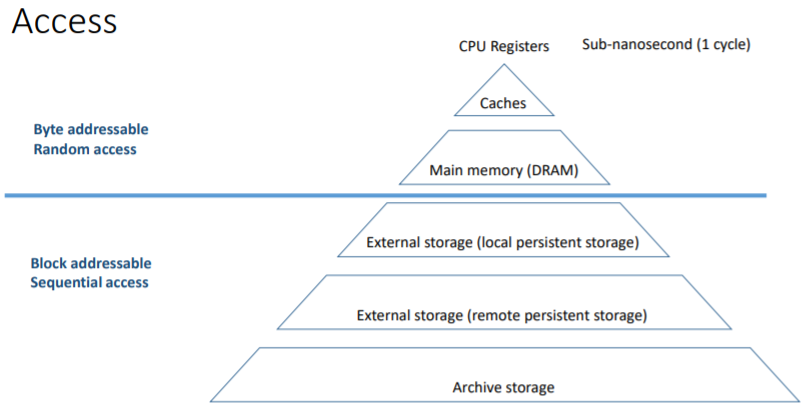
\includegraphics[scale=0.5]{images/1-acc.PNG}
	\caption{Memory hierarchy access methods.}
	\label{fig:acc}
\end{figure}

\paragraph{Memory Wall}
Main memory suffers from several issues: there is never enough of it (application growth), memory outside the CPU chip (DRAM) is much slower than memory located inside of it (latency issue), processor-memory gap (processor speed increases faster than memory speeds - bandwidth is an issue), increased cost (DRAM is expensive) and main memory is not persistent.

\paragraph{Spatial Locality}
Put together what belongs together.

\paragraph{Temporal Locality}
Do at the same time things that require the same data.

\paragraph{Non-Volatile Memory (NVM)}
Located between DRAM and local external storage - combines characteristics of both. Byte addressable, random access, persistent, etc.

\paragraph{Cloud Computing}
Network between compute and storage layer. Ephemeral nature of computing infrastructure forces a separation of compute and storage. Flexibility is provided by cloud provider.

\paragraph{Network Attached Storage (NAS)}
Networks are becoming faster with more bandwidth than storage devices (e.g. RTT in a data center less than a seek operation on a HDD). Eventually, it might be faster to get data from the memory of a remote machine / storage device than from local disk. See also: Remote Direct Memory Access (RMDA).

\paragraph{Multicore and NUMA}
%TODO potentially

\paragraph{Hardware Acceleration}

\paragraph{SSD}






\subsection{Logical Storage Organization}

See the first layer in Figure \ref{fig:arch}. Assumptions: the standard database architecture is based on slow hard drive disks (HDD) that have a high latency for seek operations (random access) - most of the DB is \textbf{not} in memory.

Disclaimer: most explanations from the lecture are based on a real system (Oracle Database)\footnote{For logical storage click \href{https://docs.oracle.com/en/database/oracle/oracle-database/19/cncpt/logical-storage-structures.html#GUID-4AF2D61A-8675-4D48-97A4-B20F401ADA16}{here} and \href{https://docs.oracle.com/cd/B19306_01/server.102/b14220/logical.htm}{here} and for disk storage click \href{https://docs.oracle.com/cd/B19306_01/server.102/b14220/physical.htm}{here} and \href{https://docs.oracle.com/en/database/oracle/oracle-database/19/cncpt/physical-storage-structures.html#GUID-008A1F08-9C75-4E9F-A70B-41FB942C60B4}{here}.}. %TODO look at these pages

Problem statement: a DB is doing many things at the same time and each thing (query, system process, DB component, etc.) active at any point in time needs its own logical view of the data. A DB creates such virtual, logical views of the system using its own mechanisms.

\paragraph{Logical and Physical Storage}
For Oracle 19, those two components are represented by an ER diagram seen in Figure \ref{fig:erdiag} with a crow foot implying a one-to-many relationship). 

A given logical object in a DB (table, index, etc.) is "stored" in a tablespace, a tablespace is organized into segments, segments have space allocated to them in the form of extents and extents are sets of contiguously allocated data blocks.

\begin{figure}[h]
	\centering
	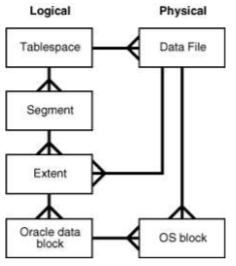
\includegraphics[scale=0.8]{images/1-erdiag.PNG}
	\caption{Oracle 19 logical vs. physical storage.}
	\label{fig:erdiag}
\end{figure}

%TODO more images?


\paragraph{Page}
There are different notions for a page:
\begin{itemize}
    \item \textbf{Hardware Pages:} The atomic unit to write to storage, usually 4KB. Also called block sometimes. Part of a file resp. disk sector.
    \item \textbf{OS Page:} The unit used by the OS to implement virtual memory, usually 4KB.
    \item \textbf{DB Page:} Equivalent to a block, anywhere between 512B and 32KB. Trend is towards larger block sizes since they incur less overhead (less keeping track).
\end{itemize}

\paragraph{Tablespace}
Data unit in a DB which provides a logical representation of the principle of spatial locality (not necessarily stored continuously!) - some form of virtual memory. Data stored is either schema related (table, index, clustered tables) or engine related (data structures for the engine, e.g. result buffers). Space (memory / disk) is allocated to tablespaces. Keep together what needs to be kept together = logical locality = one address.

\paragraph{Segment}
An object in the schema (or part of an object if it is partitioned). Consists of one or more extents (that can be in different data files). Segments allocate (virtual) space to objects. Usually when allocating space, a DBMS gives a little bit more to have some growing space. Even if a table is partitioned into several segments across various disks, the table still has only one tablespace.

\paragraph{Extent}
A collection of physically continuous data blocks (size = tunable /dynamic parameter). Extents are mapped to one data file. Usually when allocating space for an extent, a DBMS gives a little bit more to have some growing space (1.25x common).

Extents are a compromise between static file mapping and dynamic block mapping. I.e. do static mapping to a set of blocks and if more space is needed dynamically do another static mapping connected to the first one. Needs an array of pointers = extent directory (which also needs space - want to keep it small).

\paragraph{Block}
The smallest amount / unit of physical space allocation. Kinda the same thing as a page in an OS - just bigger. The block size is a tunable parameter. With a small block size, you need to keep track of many physical locations and less actual sequential access. With a big block size, you will have fragmentation but more actual sequential access.

\paragraph{Block Structure: Slotted Pages}
A block has a header (address and type of segment, e.g. index, table, etc.), a table directory (schema of the table stored in the block), row directory (pointers to the actual tuples stored in the block (block, slot), data can be anywhere), free space and row data (tuples stored in the block). The directory grows downwards and the space for the tuples grows upwards.

No assumptions can be made on storage order of a table within an extent! E.g. if a tuple is deleted a new one can take its place that has been inserted much later.

\paragraph{Optimizing Block Usage}
\begin{itemize}
    \item \textbf{Percentage Free (PCTFREE):} Allow row inserts until x\% of the space is occupied and leave the rest for updates to existing rows in the blocks. Avoids fragmentation occurring from updates that make an already existing tuple larger. 
    \item \textbf{Percentage Used (PCTUSED):} Determines how much space needs to be free before free space is used to insert new tuples. No more new inserts until used space is under x\%. Avoids having to constantly move a block from the used to the free list and vice versa (costly operation).
    \item These two concepts are often combined. They are a trade-off between efficiency and space.
\end{itemize}

\paragraph{Fragmentation Within Blocks}
Blocks can suffer from fragmentation. Compaction is expensive and only done when the block has enough space for an insert / update but the space is not contiguous. In case of an update not fitting the original block anymore, the tuple is put into a new block with a row pointer in the original space s.t. the ID of the tuple does not need to change (needs indirection) - too much of this slows down access since it multiplies I/O by a factor of at least 2.

\paragraph{Finding Space}
Segments contain one or more free lists that keep track (with pointers) of blocks that have usable free space (not done at an extent-level because the search for space would be more complex). Using several free lists helps avoid contention when performing parallel inserts / updates, e.g. different lists for different actions. Free lists are updates as transactions execute insert / delete / update statements using the rules established with Percentage Free and Percentage Used.

\paragraph{Writing to Disk}
A DB provides concurrency control (DB correct even if several transactions modified data at the same time) and recovery (data can be recovered even after a failure). More details in later sections.

\textbf{Shadow Paging:} When updating an attribute, copy it to a free slot (= page) and update it there. Once the transaction commits, mark the old slot as free and the new one as correct. Only makes sense when the overhead of creating a new copy and managing them is small enough (main memory, flash, NVM, etc.).

\textbf{Delta Files:} A copy of the attribute that is to be updated is stored in a delta file (instead of a free slot in the extent). The update is performed directly on the original value and the copy in the delta file can be discarded if it's no longer needed. Old data in delta file favors commits, simplifies undos and allows looking at older data. New data in delta file favors aborts and allows to delay the propagation of updates.\footnote{Oracle used rollback segments (segments used to store old copies of data) and now switched to undo-tablespaces.}












\subsection{Database Buffer Cache}

See second layer in Figure \ref{fig:arch}. To process data, it has to reside in memory. Since not all the data fits into memory, databases cache blocks in memory and write them back to storage when dirty or in need of more space. So, to provide efficient access to pages, a DBMS implements a large shared buffer pool in its own memory space. A buffer pool is organized as an array of frames, each of the size of a DB disk page. The buffer cache is not used for actual processing - intermediate results are stored in the database heap (region of memory where queries actually work on the data).

Similar to OS virtual memory / paging mechanisms but a DB has much better knowledge about access patterns and the process can be optimized to a larger extend.

It is important to keep the overhead of data structures in mind that are needed to keep track of things.

\paragraph{Buffer Manager}
The buffer manager does all the bookkeeping of the buffer pool and is implemented as a hash table. The table maps page numbers currently held in memory to their location in the frame table, the location for that page on disk and additional metadata associated with the page. The metadata includes a dirty bit indicating the data on the page has been modified and info needed by the chosen replacement policy (pin count, statistics, etc.).

\begin{figure}[h]
	\centering
	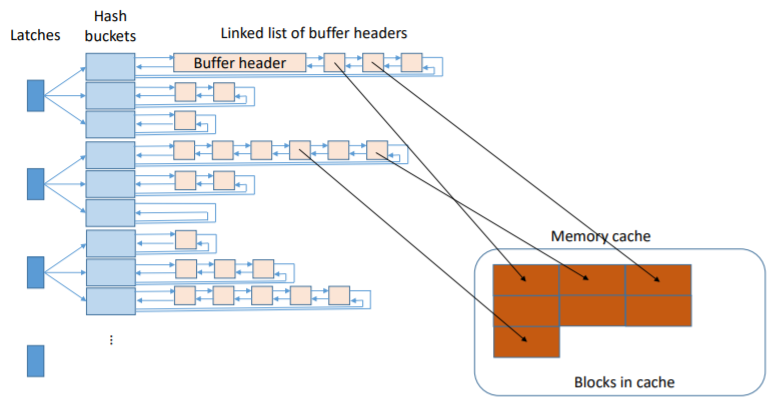
\includegraphics[scale=0.8]{images/1-buffer.PNG}
	\caption{Architecture of a DB buffer manager.}
	\label{fig:buffer}
\end{figure}

\paragraph{Hash Table}
To check if a block is in memory, we take its ID and hash it. Look up the position indicated by the resulting value to check. This is the first check we need to do when processing data.

\paragraph{Latches}
Mechanism to access hash table(s) without the risk of a conflicting concurrent access (similar to a lock)\footnote{Locks usually avoid conflicting updates to data by transactions, while latches avoid conflicting updates in system data structures.}. A latch usually covers several hash buckets (tunable parameter). Latching per bucket or even per block header results in too much overhead since there are so many.

\textbf{Performance Issues:} To check if a block is in memory, a latch needs to be acquired. Since a latch can be only owned by one process, this process blocks several linked lists of block headers. Contention on these latches may cause performance problems (hot blocks, SQL statement accessing many blocks, similar statements executed concurrently, etc.).

\textbf{Mitigation:} Reduce amount of data in the block (with PCTFREE / PCTUSED), more latches and less buckets per latch, multiple buffer pools, tune queries to minimize number of blocks accessed (avoid table scans), avoid many concurrent queries / transactions accessing same data, etc.

\paragraph{Hash Bucket}
Correct linked list storing block header is found by hashing on some form of block identifier. 

\paragraph{Buffer Header Double Linked List}
After hashing, the linked list is traversed looking for an entry (block header) for the corresponding block. Keep the lists short since this is expensive (have more buckets). A block header contains lots of info (block number, type, format, LSN, integrity checksum, latches / status flags, buffer replacement info).

Some engines store other types of blocks in the linked lists, e.g. version blocks (updates result in copies with a timestamp inserted into the list, similar to shadow paging), undo / redo blocks for recovery, dirty blocks, pinned blocks, etc.

\paragraph{Block Status}
The following states are relevant for the management of the buffer: pinned (block cannot be evicted), usage count (statistics on specific block), clean / dirty. This info is used when implementing cache replacement policies. 

\paragraph{Cache Replacement Policy}
What to cache, what to keep, how to evict and when, how to avoid thrashing cache with unnecessary traffic.

\textbf{Least Recently Used (LRU):} Keep track of when a block was used in a list - most recently used. When evicting, pick the least recently used block at the bottom. Does not work very well for DBs (in contrast to OSes) since large table / index range scans can pollute the cache without actually needing to re-access the cached data.

\textbf{Modified LRU:} Put rarely accessed data (statistics) at the bottom of the list or simply don't cache large tables. Or sort blocks according to access frequency instead of simple counters.

\paragraph{Optimizations}
\begin{itemize}
    \item Keep Buffer Pool: tell DB which blocks are important and should not be evicted (separate buffer).
    \item Recycle Buffer Pool: tell DB which blocks should not be kept after they are used (separate buffer).
    \item Keeping statistics of usage of tables and let system decide automatically what should / shouldn't be cached.
    \item Choose clean pages when needing to evict since it's faster (no write to storage).
    \item Ring Buffers: for scans, allocate the pages in a ring s.t. blocks are allocated only within the ring. Full buffer - evict pages from beginning of the ring as they have already been scanned.
    \item Since block sizes are not homogeneous, require a buffer cache for each block size for more space efficient replacement and simple management.
\end{itemize}

%TODO p. 24, read ahead and stuff, interactions

\paragraph{Touch Count (Hot / Cold List)}
A more sophisticated LRU. Insert new blocks in the middle of the list and keep a count of accesses. Frequently accessed blocks float to the top while rarely accessed ones sink. To avoid counting problems (many accesses only for a short amount of time), only increment counter after a (tunable) number of seconds. Periodically decrease counters.

\paragraph{Second Chance}
Strategies similar to LRU can become a bottleneck if the lists are large. With second chance, no list is maintained and counters are kept in the blocks. Buffer is treated as a circular buffer with an eviction process going around. When a page is accessed, counter = 1. When eviction process passes, if counter is 1, set to 0 - if 0, evict page.

\paragraph{Clock Sweep}
Same as second chance but takes into account that some pages are accessed frequently at regular intervals - uses a counter (with tunable max) instead of a 1/0 flag. Increase counter when touched, decrease when eviction passes, evict when counter = 0.

\paragraph{2Q: Using Two Lists}
Use a FIFO list for blocks that do not need to be kept and a LRU list for blocks that are accessed several times. If a block in the FIFO list is accessed again, it is moved to the LRU list. Blocks at the bottom of the LRU list are either moved to FIFO list (or immediately evicted). Evictions happen on FIFO list level.



\subsection{Storage Techniques in Context}

Instead of using physical storage, we are now looking at using a cloud storage and file system (such as Amazon S3). The previous material is put into context with a modern example of a database, namely \textit{Snowflake}.

\paragraph{Snowflake}
A data warehouse specialized for analytical queries developed entirely on the cloud (cloud native). Separates compute (nodes running VMs with a local disk) from storage (Amazon S3).

The query processing layer (compute) is made up of virtual warehouses, with each consisting of a collection of worker nodes (EC2 instances in Amazon). Each worker node has a cache in its local disk with a simple LRU replacement policy. Metadata in the cloud services level tells us where things are stored. %TODO right?

\begin{figure}[h]
	\centering
	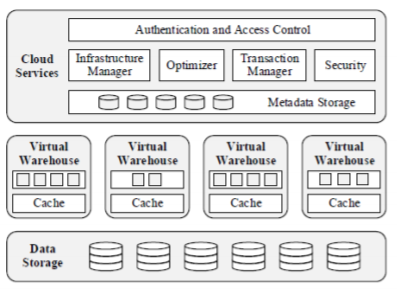
\includegraphics[scale=0.8]{images/1-snowflake.PNG}
	\caption{Snowflake architecture.}
	\label{fig:snowflake}
\end{figure}

\paragraph{Amazon S3 (Simple Storage Service)}
Object storage service in the cloud that acts as he persistent storage that is available to applications. Unlike conventional local disks / distributed file systems (key-value where every object has a key, HTTP(S) PUT / GET / DELETE interface, no updates in place - only full writes that replace old object, can read parts of an object, high CPU overhead because of HTTP, extra expensive I/O because it's network based).
%TODO more?

\paragraph{Micro-Partitions}
Snowflake's extents. To facilitate query processing, they are organized in a special way:

\begin{itemize}
    \item Size ranges between 50 and 500 MB (before compression - data always compressed in S3). In contrast in other DBs, extents are typically in the order of KB.
    \item Each micro-partition has metadata describing what's inside.
    \item Metadata can be read without reading the whole micro-partition.
    \item Metadata is used to read just the part of the micro-partition that is relevant.
    \item Data in micro-partition is stored in columnar form (not by rows). This is the preferred storage format for analytics, improves cache locality, enables vectorized processing, facilitates projection operations and allows to process only the part of the table that is relevant.
    \item Horizontal partitioning (table partitioned into several MP horizontally) - allows to read the table in parallel and facilitates reading only wanted info.
    \item All of this allows for storage level processing to read only parts of the file that are needed which minimizes data movement to and from storage.
\end{itemize}

\begin{figure}[h]
	\centering
	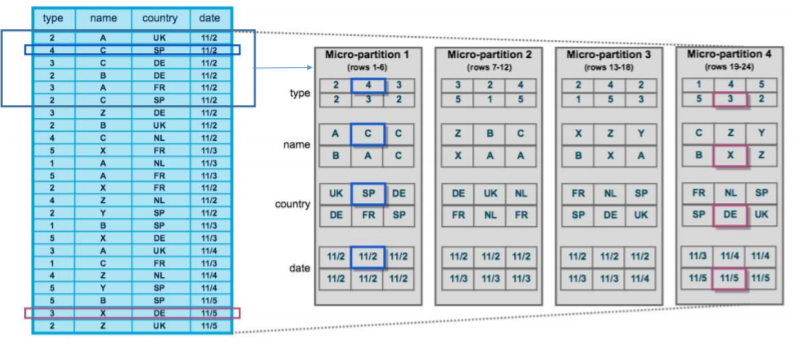
\includegraphics[scale=0.8]{images/1-micropart.PNG}
	\caption{Logical and physical table structure in Snowflake.}
	\label{fig:micropart}
\end{figure}


\paragraph{Pruning based on Metadata}
Example of metadata: in this MP the min. age is x and the max age is y. With a query only wanting all entries with age $>$ y, we can discard that MP. Other examples are: number of distinct values, number of nulls, bloom filters, etc.

Snowflake does not use indexes (requires a lot of space, induce random accesses which are bad for slow storage like S3, need to be maintained and selected correctly). Metadata is much smaller and easier to load.

\paragraph{Writing to Disk}
S3 does not support in-place updates (immutable), an object is replaced in its entirety. Snowflake uses this to implement snapshots of the data (shadow paging): write a new object when MP is modified and keep / discard old MP. Allows for reading of old data and provides fault-tolerance.



\subsection{Reading Assignments}

\subsubsection{An Evaluation of Buffer Management Strategies for Relational Database Systems}

Again: data has to be in RAM for a DBMS to operate on it! A buffer manager intelligently shuffles data from disk to memory. A buffer pool contains frames that can hold pages brought in from disk and are otherwise free. The pool is filled according to some kind of algorithm and replacement policy. A pinned page is a page currently in use - it should not be replaced. Pages that contain modified data are dirty and need to be written back to disk before discarding them.

\paragraph{Domain Separation Algorithm}
Why? Not all pages are the same! Pages are statically classified into types. If a page of type X is needed, allocate it in pool X = domain X. A pool contains several buffers = slots to put the requested pages into. In each domain, LRU is used as the replacement policy. If no slots are available in current domain, borrow slots from another domain.

A suggested type assignment scheme is: assign one domain to each non-leaf level of a B-Tree structure while all the leaves and their data also get one domain.

Cons: Domains are a static concept - the importance of a page may vary across queries - relative importance matters. Partitioning buffers according to domains rather than queries does not prevent interference among competing users. Thrashing is still an issue, there is no load control. There are no priorities among domains (e.g. index page $>$ data page).

\paragraph{Group LRU Algorithm}
The above but with a fixed priority ranking among different groups = domains. Searching for free space always starts at domain with lowest prio.

\paragraph{DS with Working-Sets}
The above but each domain can dynamically vary in size - working-set-like partitioning scheme. Pages in domain i which have been referenced in the last t\_i references are exempt from replacement consideration.

\paragraph{Page-Type Algorithms}
All of the above - TL;DR: they're shit and not really superior to simple LRU or CLOCK.

\paragraph{"New" Algorithm}
Shittiest name ever by the way. Two key observations: The priority of a page is not a property of the page; in contrast, it is a property of the relation to
which that page belongs. Each relation should have a Working Set. 

Buffer pool is subdivided and allocated per-relation. Each relation with buffered pages has a resident set = all buffered pages - replacement policy within each is MRU. Each active relation is entitled to one pinned buffer. Resident sets are linked in a priority list with a global free list on top. High priority (based on some heuristic) is at bottom and less likely to be replaced than top since search for free space starts at top.

Cons: MRU. How to assign prios? List search. No regard for multi-user use case. TL;DR: it has a shitty name AND it is shitty. It's 2 AM and I'm tired.

\paragraph{Hot Set Algorithm}
Hot set: set of pages over which there is a looping behavior - keep those in memory by allocating a large enough buffer pool. Hot point: plot buffer size vs. number of page faults and observe that at some point the buffer is too small and MRU/LRU is shit which equates to lots of page faults. E.g. nested loop join with seq. scan: hot point = number of pages in inner relation plus one.

Hot points for different kinds of queries can be determined but it depends on replacement algo (MRU works better than LRU sometimes, especially in cyclic loops).

Query receives hot points amount of buffers. New query can only enter the system if there's enough space for it according to its hot set size. Leads to memory under-utilization due to overallocation.

\paragraph{Query Locality Set Model (QLSM)}
A RDBMS supports a limited set of operations and the pattern of page references they exhibit are regular and predictable. Each pattern can be decomposed into a number of simple reference patterns. With this, the size of a locality set can be determined in advance per query (= set of buffered pages associated with a file instance = multiple pages belonging to same table). %TODO examples below, check notes for reference patterns

\textbf{Sequential References:} Pages are referenced and processed one after another. \textbf{Straight sequential (SS):} sequential scan without repetition, set = 1. \textbf{Clustered sequential (CS):} clusters made up of records with same key are scanned multiple times, buffer should keep clusters until scan moves on to next cluster, set = number of records in largest cluster divided by numbers of records per page (blocking factor), FIFO and LRU work best. \textbf{Looping sequential (LS):} repeated sequential scan, buffer needs to keep entire file and if it's too large use MRU, set = total number of pages in the file.

\textbf{Random References:} \textbf{Independent random (IR):} data pages are accessed in a random manner. \textbf{Clustered random (CR):} random accesses of clusters, set = number of records in largest cluster. %IR TODO

\textbf{Hierarchical References:} Sequence of page accesses forming a traversal path from root to leaves of an index. \textbf{Straight hierarchical (SH):} index is traversed only once, one buffer frame is enough, set = 1. \textbf{Hierarchical SS (H/SS):} tree traversal with sequential scan of the leaves, set = 1. \textbf{Hierarchical CS (H/CS):} tree traversal with clustered sequential scan of the leaves, set = same as in CS, but replace record with key-pointer pair. \textbf{Looping hierarchical (LH):} repeated access to index structure, pages closer to root are accesses more frequently. %TODO LH

\paragraph{DBMIN}
See extra notes.







\subsubsection{Native Storage Extension for SAP HANA}

\paragraph{SAP HANA}
Column-oriented in-memory DBMS combining OLTP and OLAP with the possibility to also use row-store. It uses multiversion concurrency control (MVCC) to manage concurrency.

\paragraph{SAP HANA with NSE}
Basically the memory-disk model that we have seen until now. Cold data on disk, hot data in memory, warm data in buffer pool.






\subsubsection{The Snowflake Elastic Data Warehouse}










\subsection{Exercises}

\subsubsection{DBMIN}
% IMPORTANT
